
\chapter{Einleitung und Motivation}%
\label{chap:Einleitung}%

Autonomous Vehicle technology has the potential to significantly improve road safety, future mobility and even our climate. Human error is responsible for about 94\% of all fatal car accidents in the US \cite{1}. This highlights a fundamental limitation in human capability to safely operate motor vehicles. ADAS has already contributed to reducing accident frequency in the UK by up to 23\% \cite{masello_road_2022}, demonstrating the great potential of automation on the road. 
By introducing fully autonomous vehicles that no longer rely on human input, tremendous safety improvements could be achieved. This could save about 29000 lives every year in the Unites States alone and would be projected to save more than 10 million lives per decade wordwide and make it one of the most important health advances in the 21st century \cite{2}. 

\begin{figure}[htbp]
    \centering
    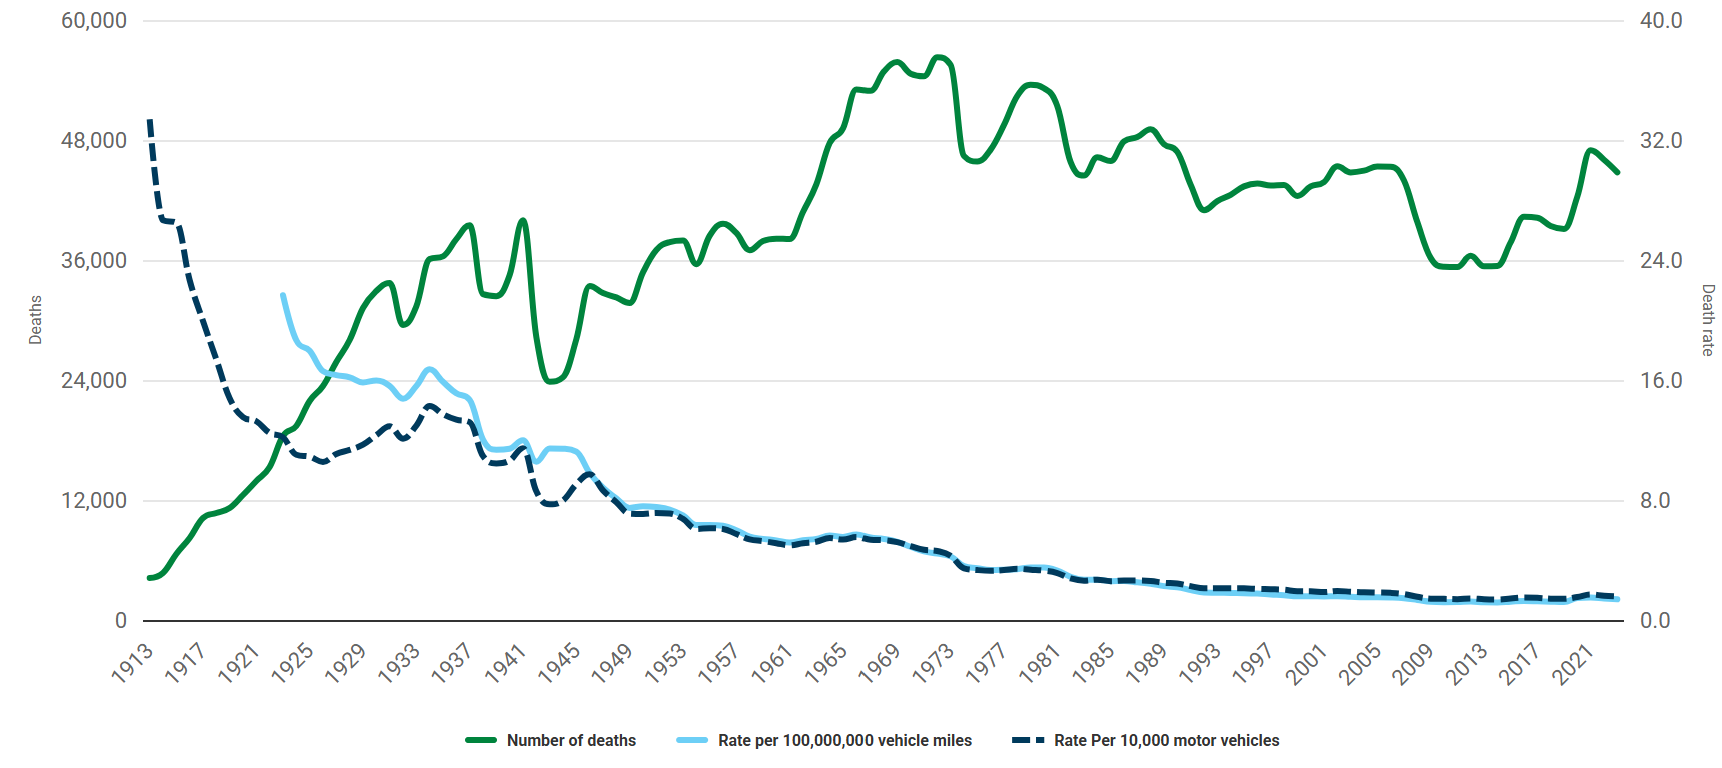
\includegraphics[scale=0.7]{figures/Figure1_3_DeathRate.png}
    \caption{%
    \textbf{Historical trends in motor-vehicle fatalities and fatality rates in the United States from 1913 to 2023, showing increasing absolute deaths alongside a strong long-term decline in deaths per vehicle and per distance traveled, reflecting improvements in road safety and vehicle technology Adapted from \cite{noauthor_historical_nodate}.
    }}
    \label{fig:figure_1_2}
\end{figure}

Despite significant improvements in vehicle technology and safety systems, fatalities caused by motor vehicle accidents remain a major global problem. As shown in Figure 1.1, there are approximately 48,000 traffic-related deaths in the United States each year, and this figure is increasing overall.

While the fatality rate per 100,000 inhabitants and per 10,000 registered vehicles has steadily declined, indicating substantial improvements in vehicle and traffic safety, this reduction has not kept pace with the growing number of vehicles on the road. Consequently, total fatalities continue to rise. This demonstrates that further safety advancements are required to compensate for increased traffic volume, as current Advanced Driver Assistance Systems (ADAS) alone are insufficient to reverse the upward trend in absolute deaths.

As around 94\% of these fatalities are caused by human error, there is significant potential to reduce both the fatality rate per 100,000 vehicles and the total number of traffic-related deaths further.

Beyond safety and driving technology, AVs could potentially lead to drivers having up to 50 minutes per day in additional time, by removing the need to physically drive a car. Instead, occupants can now work, rest or do other things. This could lead to up to 50 minutes per day in spare time per driver, which could potentially free up to one billion hours of time globally and therefore increase productivity and revenue for services used during that time. Additionally cities could be transformed into more livable spaces, by removing and shrinking many parking spaces and possibly roads. \cite{3}. 

In parallel, widespread AV adoption could reshape urban mobility. Reduced reliance on privately owned vehicles and increase usage of vehicles through shared mobility concepts. Optimized traffic  flow as well as driving behaviour could also improve enviornmental issues with the current automotive indsutry.

\begin{figure}[htbp]
    \centering
    
\includegraphics[scale=0.8]{Fugure_1_1_Mckinsey.png}
    \caption{%
    \textbf{Descriptive title of the figure that actually explains what the reader is looking at.
    Source: Adapted from \cite{3}.
    }}
    \label{fig:figure_1_2}
\end{figure}


Currently, the development is in phase 1, and Companies such as Waymo or Tesla with their Robotaxi division have rolled out and can be used by the general public, creating a first touch point with autonomous vehicles.
Ensuring the safety and resilience of AVs is critical for achieving public
acceptance. Perception sensors, such as LiDAR, cameras,
and radar, are central to this goal because they provide fundamental data for perception, localization, mapping, and control. LiDAR is specifically emerging as the dominant sensor, as the automotive and industrial LiDAR market is expected to exceed 6 billion USD by 2027. This presents a compound annual growth rate of 22\%, which is driven by the automotive industry and highlights the growing importance of LiDAR and AVs \cite{noauthor_china_2022}. 

However, recent studies have shown that AVs are highly vulnerable to sensor
degradation, particularly under adverse environmental conditions, such as fog or heavy
rain. These conditions distort sensor measurements asymmetrically, causing LiDAR and
other systems to reach their operational limits. Consequently, localization and perception
algorithms may fail to maintain accurate vehicle pose estimation or conduct accurate
object detection and classification, resulting in unsafe behavior. Several papers suggest that, in case of a LiDAR localization fault, the system will transition to a "fail-safe" or "fail-degraded" state. This means the vehicle will either pull over and relinquish control to the driver or continue operating with limited capabilities [Fault Tolerance and Fallback strategies].

Knowing that adverse environmental conditions can cause sensor degradation, it is
important to create robust algorithms and test these against edge cases in order to ensure
safe operation under these conditions. Doing this presents a challenge, as real-world
testing is statistically infeasible, as it would require driving billions of kilometers to observe
enough corner cases and adjust the algorithms \cite{kalra_driving_2016}. Therefore, simulation-based fault
injection, which is recommended by ISO 26262, has emerged as a powerful method for
systematically identifying and evaluating rare, safety-critical situations.

\begin{figure}[htbp]
    \centering
    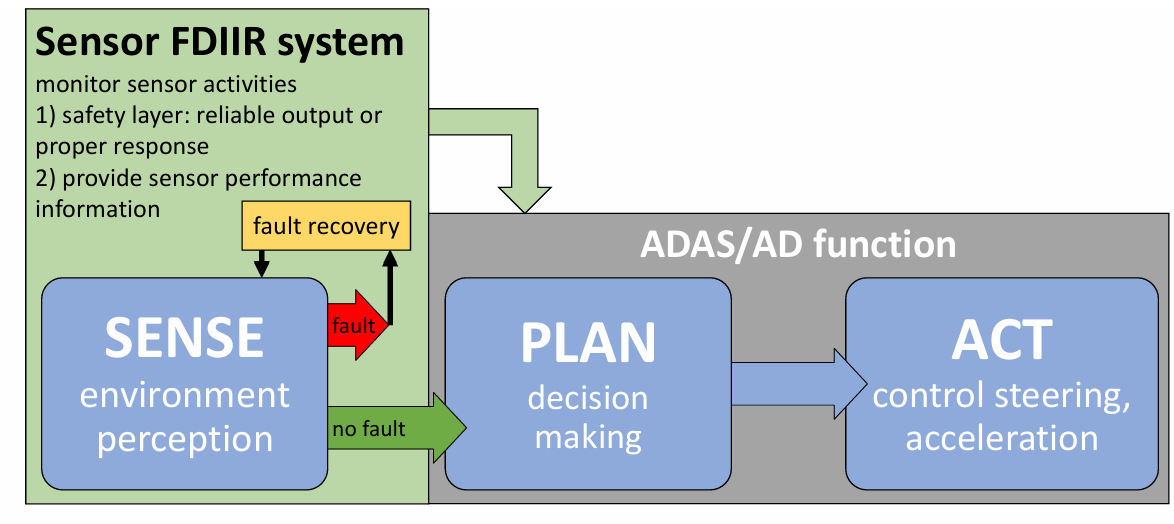
\includegraphics[scale=1]{figures/Figure_1_2_SensePlanAct.png}
    \caption{%
    \text{Schematic illustration of the sense-plan-act cycle including a sensor FDIIR (fault detection,
isolation, identification, and recovery) system that monitors the sensor activity to ensure a reliable
environment perception.
    Source: Adapted from \cite{goelles_fault_2020}.
    }}
    \label{fig:figure_1_2}
\end{figure}


Within the modular Sense–Plan–Act architecture, perception modules convert raw sensor data into geometric or semantic representations to support localisation. The localisation module then estimates the vehicle’s pose, a critical state input for downstream planning and control algorithms (see Figure 1.1).

As the localization subsystem provides all downstream modules with the vehicle’s state estimate, any degradation in its performance, such as sensitivity to adverse weather conditions, propagates through the entire sense–plan–act pipeline. Therefore, it is crucial to carefully stress-test the localisation subsystem under environmental perturbations.

Faults originating from sensor disturbances or perception errors will therefore propagate through this chain if not properly handled, ultimately leading to unsafe decisions or collisions.
Therefore, assessing the robustness of localization algorithms, particularly the LiDAR data, under such faulty conditions is essential for the safety validation of autonomous vehicles. 


As LiDAR has become the primary sensing sensor for vehicle localisation, it is essential to understand the impact of sensor degradation under adverse weather conditions on localisation performance in order to ensure the safe operation of autonomous vehicles. This thesis presents a probabilistic fault injection framework that applies controlled perturbations to LiDAR point clouds, evaluating their effect on localisation accuracy using the KISS-ICP algorithm.

This framework is highly relevant to industrial validation as well as academic research, as existing approaches hardly offer a systematic way to quantify localisation sensitivity to faults at the sensor level.

The goal is to be able to determine under which conditions it will still be possible to continue the safe operations, before needing to stop. 

